\documentclass[dvipdfmx]{standalone}
\usepackage{tikz}
\usetikzlibrary{matrix}

\tikzset{
1/.style={fill=red!30},
2/.style={fill=blue!30},
3/.style={fill=orange!30},
4/.style={fill=green!30},
5/.style={fill=red},
arrow/.style={thick,->,>=stealth},
}

\begin{document}
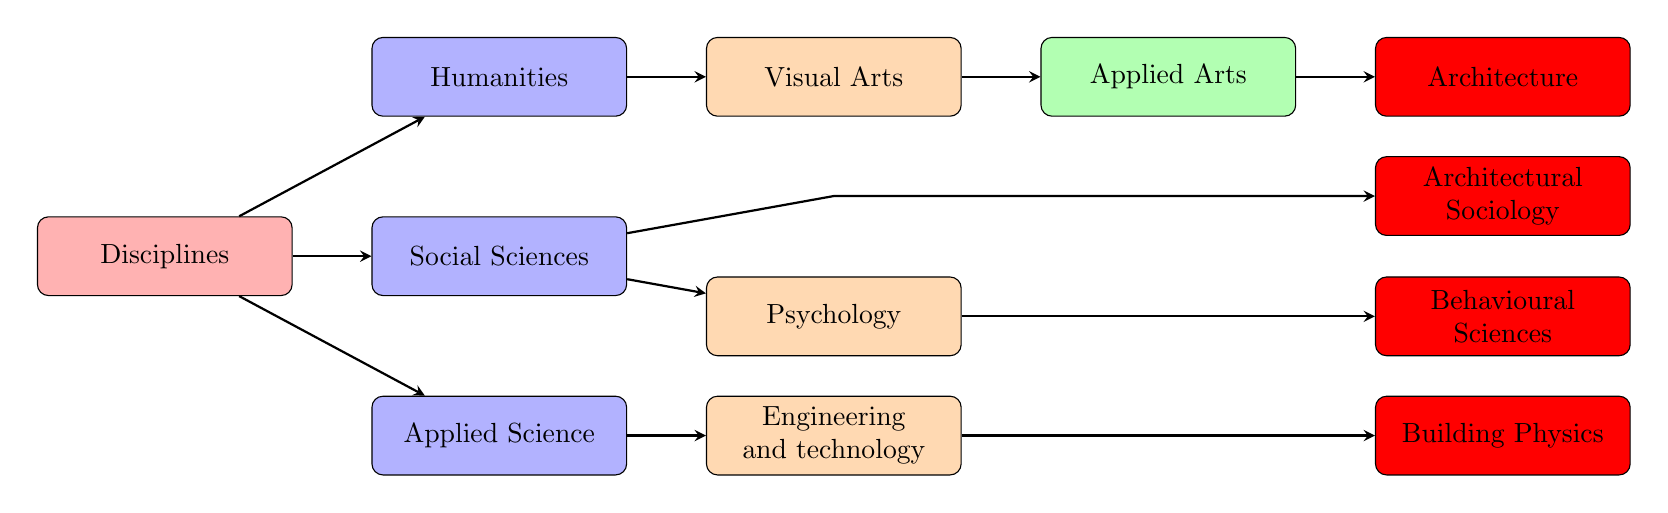
\begin{tikzpicture}
\matrix(m)[matrix of nodes,column sep=1cm, row sep=0.5cm,
nodes={rectangle, rounded corners, text width=3cm, minimum height=1cm,text centered, draw=black,anchor=west},
]{
 & \node[2](humanities){Humanities}; &\node[3](visual_arts){Visual Arts}; & \node[4](applied_arts){Applied Arts}; & \node[5](architecture){Architecture};\\
 &  & \node[draw=none](int){}; & & \node[5](sociology){Architectural Sociology};\\[-0.75cm]
\node[1](disciplines){Disciplines}; &\node[2](social_sciences){Social Sciences}; & & &\\[-0.75cm]
 &   & \node[3](psychology){Psychology}; & & \node[5](behavioural_sciences){Behavioural Sciences};\\
& \node[2](applied_sciences){Applied Science}; & \node[3](engineering_and_tech){Engineering and  technology}; & & \node[5](building_physics){Building Physics};\\
};

\draw [arrow] (disciplines) -- (humanities);
\draw [arrow] (humanities) -- (visual_arts);
\draw [arrow] (visual_arts) -- (applied_arts);
\draw [arrow] (applied_arts) -- (architecture);

\draw [arrow] (disciplines) -- (social_sciences);
\draw [arrow] (social_sciences) --(int.center)-- (sociology);
\draw [arrow] (social_sciences) -- (psychology);
\draw [arrow] (psychology) -- (behavioural_sciences);

\draw [arrow] (disciplines) -- (applied_sciences);
\draw [arrow] (applied_sciences) -- (engineering_and_tech);
\draw [arrow] (engineering_and_tech) -- (building_physics);
\end{tikzpicture}
\end{document}